\documentclass[12pt,letterpaper]{article}
\usepackage[spanish,es-nodecimaldot]{babel}
\usepackage[utf8]{inputenc}
\usepackage[T1]{fontenc}
\usepackage{float}

%% Sets page size and margins
\usepackage[a4paper,top=2.5cm,bottom=2.5cm,left=2cm,right=2cm]{geometry}

\usepackage{amsmath}
\usepackage{amssymb}
\usepackage{amsthm}
\usepackage{mathtools}
\usepackage{float}
\usepackage[colorinlistoftodos]{todonotes}

%Author affil
\usepackage{authblk}


%% Title
\title{
		\vspace{-0.7in} 	
		\usefont{OT1}{bch}{b}{n}
		\begin{minipage}{3cm}
        \vspace{-0.5in} 	
    	\begin{center}
    		
\includegraphics[height=3.2cm]{../logo_unam.png}
    	\end{center}
    \end{minipage}\hfill
    \begin{minipage}{10.7cm}
    
    	\begin{center}
\normalfont \normalsize \textsc{UNIVERSIDAD NACIONAL AUTÓNOMA DE MÉXICO \\ FACULTAD DE CIENCIAS \\ Organización y Arquitectura de Computadoras } \\
		\huge Tarea 02
    	\end{center}
     
    \end{minipage}\hfill
    \begin{minipage}{3.2cm}
    \vspace{-0.5in} 
    	\begin{center}
    		
\includegraphics[height=3.2cm]{../logo_fc.png}
    	\end{center}
    \end{minipage}

\author{Nieto Gallegos Isaac Julian}
\date{319021518}
}

 \setlength {\marginparwidth }{2cm}
 
\begin{document}

\maketitle

\textbf{Instrucciones:} Entregar por classroom en \LaTeX, escribir su nombre y número de cuenta en su tarea, la tarea es individual. Para los incisos de circuitos habrá un assignment en el grupo de CircuitVerse donde podrán hacer la entrega de todos sus circuitos. \textbf{Favor de hacer un subcircuito por cada inciso.}\\

Ejemplo:
\begin{figure}[h]
    \centering
    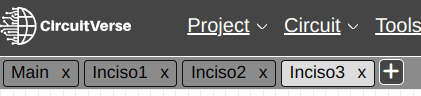
\includegraphics[width=0.75\linewidth]{A.png}
\end{figure}

% \input{Tarea01/t01}
% \begin{enumerate}
    \item Escribe en base 10 qué número representan las siguientes cadenas de 8 bits con las distintas representaciones. (2 puntos).

    \begin{table}[H]
    \begin{tabular}{|l|l|l|l|l|l|}
    \hline
             & \begin{tabular}[c]{@{}l@{}}Entero\\ sin signo\\ (natural)\end{tabular} & \begin{tabular}[c]{@{}l@{}}Entero con\\ bit de signo\end{tabular} & \begin{tabular}[c]{@{}l@{}}Entero con\\ offset, con un\\ desplazamiento\\ de -40\end{tabular} & \begin{tabular}[c]{@{}l@{}}Complemento\\ a 1\end{tabular} & \begin{tabular}[c]{@{}l@{}}Complemento\\ a 2\end{tabular} \\ \hline
    00000000 &                                                                        &                                                                   &                                                                                               &                                                           &                                                           \\ \hline
    10101010 &                                                                        &                                                                   &                                                                                               &                                                           &                                                           \\ \hline
    11110000 &                                                                        &                                                                   &                                                                                               &                                                           &                                                           \\ \hline
    10000000 &                                                                        &                                                                   &                                                                                               &                                                           &                                                           \\ \hline
    01111111 &                                                                        &                                                                   &                                                                                               &                                                           &                                                           \\ \hline
    \end{tabular}
    \end{table}

    \item Diseña e implementa las funciones que se piden en el código adjunto.
    
\end{enumerate}
\section*{Circuitos}

\begin{enumerate}
    \item Demuestra que las compuertas NAND y NOR son universales (2 puntos)
    \item Dado que ya sabes implementar un Half Adder (HA) utilizando compuertas lógicas, ahora debes diseñar e implementar un Full Adder (FA) combinando dos Half Adders y una compuerta OR. (3 puntos)
    \begin{enumerate}
        \item Usa dos Half Adders para sumar los bits de entrada A y B junto con el bit de acarreo de entrada $C_{in}$.
        \item Usa una compuerta OR para combinar los acarreo intermedios y obtener el $C_{out}$.
        \item Implementa el circuito usando compuertas lógicas básicas.
        \item \textbf{Entrega en tu PDF} la expresión booleana simplificada del Full Adder.
    \end{enumerate}
    \item Implementa el full adder usando únicamente compuertas NAND (3 puntos)
    \item Da la expresión lógica asociada a la siguiente tabla de verdad usando su forma canónica disyuntiva, luego minimiza esa expresión usando mapas de Karnaugh e implementa un circuito equivalente a esa expresión. (Adjunta el mapa de Karnaugh a la tarea). (2 puntos).

    \begin{table}[H]
    \centering
    \begin{tabular}{|l|l|l|l|l|}
    \hline
    X & Y & Z & W & Output \\ \hline
    0 & 0 & 0 & 0 & 0      \\ \hline
    0 & 0 & 0 & 1 & 1      \\ \hline
    0 & 0 & 1 & 0 & 0      \\ \hline
    0 & 0 & 1 & 1 & 0      \\ \hline
    0 & 1 & 0 & 0 & 0      \\ \hline
    0 & 1 & 0 & 1 & 1      \\ \hline
    0 & 1 & 1 & 0 & 1      \\ \hline
    0 & 1 & 1 & 1 & 1      \\ \hline
    1 & 0 & 0 & 0 & 0      \\ \hline
    1 & 0 & 0 & 1 & 0      \\ \hline
    1 & 0 & 1 & 0 & 1      \\ \hline
    1 & 0 & 1 & 1 & 0      \\ \hline
    1 & 1 & 0 & 0 & 1      \\ \hline
    1 & 1 & 0 & 1 & 0      \\ \hline
    1 & 1 & 1 & 0 & 1      \\ \hline
    1 & 1 & 1 & 1 & 0      \\ \hline
    \end{tabular}
    \end{table}

    
\end{enumerate}

\end{document}
